\documentclass{article} % For LaTeX2e
\usepackage{../../tex-style/nips_2014,times}
\usepackage{hyperref}
\usepackage{url}
\usepackage{graphicx}
\usepackage{CJKutf8}
\hypersetup{unicode}
\AtBeginShipoutFirst{\input{zhwinfonts.tex}}
\usepackage{algorithm}  
\usepackage{algorithmic}
\usepackage{amsmath}
\title{Learning Deep Structured Semantic Models for Web Search Using Clickthrough Data}

\author{
 \url{https://www.dosrc.com/}
}


\nipsfinalcopy % Uncomment for camera-ready version

\begin{document}
\begin{CJK*}{UTF8}{gkai}

\maketitle

\section{相关知识}
\subsection{LSA}
LSA(latent semantic analysis):潜在语义分析
传统向量空间模型使用词语匹配,无法解决同义词和多义词的导致检索精确度的下降的问题,所以需要语义层面的分析匹配

\subsubsection{LSA的步骤如下:}

1. 分析文档集合,建立Term-Document矩阵。

2. 对Term-Document矩阵进行奇异值分解。

3. 对SVD分解后的矩阵进行降维,也就是奇异值分解一节所提到的低阶近似。

4. 使用降维后的矩阵构建潜在语义空间,或重建Term-Document矩阵。


\section{背景}
从LSA发展而来的概率主题模型(probabilistic topic models)例如probabilistic LSA (PLSA)和Latent Dirichlet Allocation (LDA)也用来做语义匹配,但是它们在网页搜索任务上的效果并没有预期的那么好。

最近研究的扩展潜在语义模型主要有两条路线。

一个是利用\textbf{clickthrough data}(将查询词语和点击的文档关联起一个数据结构)作为训练数据,例如Bi-Lingual Topic Models (BLTMs) 和 linear Discriminative Projection Models (DPMs),
BLTM通过最大化似然函数而不是直接优化排名得到的结果是次优的。DPM训练中有大量的矩阵乘法,并且矩阵的维数随着词汇量的增加而显著增加,在web搜索中能达到百万级别,尽管可以通过修剪词汇量让训练时间得以让人忍受,但是结果也是次优的。

一个是Salakhutdinov 和 Hinton的\textbf{深度自编码器},深度自编码器的参数优化主要是为了重建文档而不是为了查询的精确度,而且为了使得训练时间可以接收,文档的词向量只使用了常见的2000个词汇。

\section{Deep Structured Semantic Models For Web Search}

\begin{center}
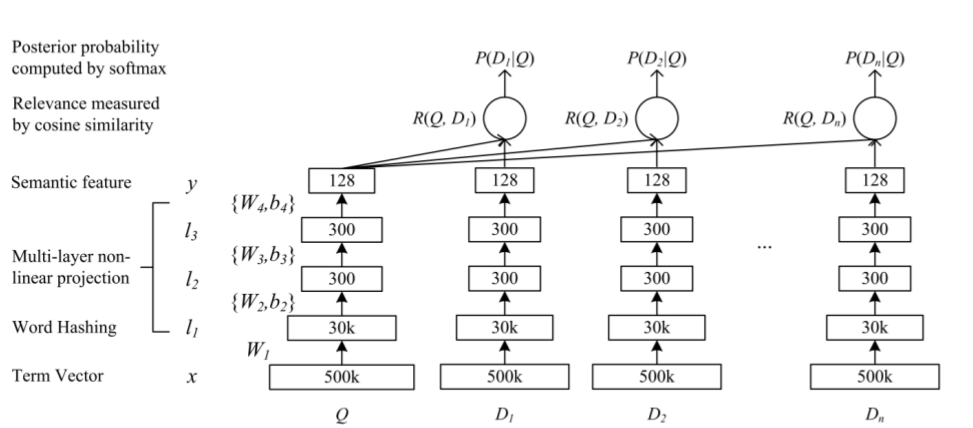
\includegraphics[width=6in]{deep-structured-semantic-models-for-web-search.png}
\end{center}
为了减少输入向量的维度,引入了word hash方法,word hash将单词用n-gram的方式表示,然后句子就可以用这些n-gram后的单词而不是原来的单词作为维度,尽管会存在一些碰撞,但是可以显著减小输入向量的维数。
值得注意的是第一层的参数是固定的是为了转化成n-gram,接下来使用clickthrough data训练整个模型,在每个query和clicked document对,在documnet中加入四个未点击的文档,训练的任务就是最大化输出已点击文档的概率。
\end{CJK*}
\end{document}